%%%%%%%%%%%%%%%%%%%%%%%%%%%%%%%%%%%%%%%%%
% Journal Article
% LaTeX Template
% Version 1.3 (9/9/13)
%
% This template has been downloaded from:
% http://www.LaTeXTemplates.com
%
% Original author:
% Frits Wenneker (http://www.howtotex.com)
%
% License:
% CC BY-NC-SA 3.0 (http://creativecommons.org/licenses/by-nc-sa/3.0/)
%
%%%%%%%%%%%%%%%%%%%%%%%%%%%%%%%%%%%%%%%%%

%----------------------------------------------------------------------------------------
%  PACKAGES AND OTHER DOCUMENT CONFIGURATIONS
%----------------------------------------------------------------------------------------

\documentclass[twoside]{article}\usepackage[]{graphicx}\usepackage[]{color}
%% maxwidth is the original width if it is less than linewidth
%% otherwise use linewidth (to make sure the graphics do not exceed the margin)
\makeatletter
\def\maxwidth{ %
  \ifdim\Gin@nat@width>\linewidth
    \linewidth
  \else
    \Gin@nat@width
  \fi
}
\makeatother

\definecolor{fgcolor}{rgb}{0.345, 0.345, 0.345}
\newcommand{\hlnum}[1]{\textcolor[rgb]{0.686,0.059,0.569}{#1}}%
\newcommand{\hlstr}[1]{\textcolor[rgb]{0.192,0.494,0.8}{#1}}%
\newcommand{\hlcom}[1]{\textcolor[rgb]{0.678,0.584,0.686}{\textit{#1}}}%
\newcommand{\hlopt}[1]{\textcolor[rgb]{0,0,0}{#1}}%
\newcommand{\hlstd}[1]{\textcolor[rgb]{0.345,0.345,0.345}{#1}}%
\newcommand{\hlkwa}[1]{\textcolor[rgb]{0.161,0.373,0.58}{\textbf{#1}}}%
\newcommand{\hlkwb}[1]{\textcolor[rgb]{0.69,0.353,0.396}{#1}}%
\newcommand{\hlkwc}[1]{\textcolor[rgb]{0.333,0.667,0.333}{#1}}%
\newcommand{\hlkwd}[1]{\textcolor[rgb]{0.737,0.353,0.396}{\textbf{#1}}}%

\usepackage{framed}
\makeatletter
\newenvironment{kframe}{%
 \def\at@end@of@kframe{}%
 \ifinner\ifhmode%
  \def\at@end@of@kframe{\end{minipage}}%
  \begin{minipage}{\columnwidth}%
 \fi\fi%
 \def\FrameCommand##1{\hskip\@totalleftmargin \hskip-\fboxsep
 \colorbox{shadecolor}{##1}\hskip-\fboxsep
     % There is no \\@totalrightmargin, so:
     \hskip-\linewidth \hskip-\@totalleftmargin \hskip\columnwidth}%
 \MakeFramed {\advance\hsize-\width
   \@totalleftmargin\z@ \linewidth\hsize
   \@setminipage}}%
 {\par\unskip\endMakeFramed%
 \at@end@of@kframe}
\makeatother

\definecolor{shadecolor}{rgb}{.97, .97, .97}
\definecolor{messagecolor}{rgb}{0, 0, 0}
\definecolor{warningcolor}{rgb}{1, 0, 1}
\definecolor{errorcolor}{rgb}{1, 0, 0}
\newenvironment{knitrout}{}{} % an empty environment to be redefined in TeX

\usepackage{alltt}

\usepackage{lipsum} % Package to generate dummy text throughout this template

\usepackage[sc]{mathpazo} % Use the Palatino font
%\usepackage[T1]{fontenc} % Use 8-bit encoding that has 256 glyphs
\usepackage[utf8]{inputenc}
\linespread{1.05} % Line spacing - Palatino needs more space between lines
\usepackage{microtype} % Slightly tweak font spacing for aesthetics

\usepackage[hmarginratio=1:1,top=32mm,columnsep=20pt]{geometry} % Document margins
\usepackage{multicol} % Used for the two-column layout of the document
\usepackage[hang, small,labelfont=bf,up,textfont=it,up]{caption} % Custom captions under/above floats in tables or figures
\usepackage{booktabs} % Horizontal rules in tables
\usepackage{float} % Required for tables and figures in the multi-column environment - they need to be placed in specific locations with the [H] (e.g. \begin{table}[H])
\usepackage{hyperref} % For hyperlinks in the PDF
\usepackage{graphicx}

\usepackage{lettrine} % The lettrine is the first enlarged letter at the beginning of the text
\usepackage{paralist} % Used for the compactitem environment which makes bullet points with less space between them

\usepackage{color} % used to mark parts that need to be edited
\usepackage{natbib} %to use citealt citet citep
\usepackage{abstract} % Allows abstract customization
\renewcommand{\abstractnamefont}{\normalfont\bfseries} % Set the "Abstract" text to bold
\renewcommand{\abstracttextfont}{\normalfont\small\itshape} % Set the abstract itself to small italic text

\usepackage{titlesec} % Allows customization of titles
\renewcommand\thesection{\Roman{section}} % Roman numerals for the sections
\renewcommand\thesubsection{\Roman{subsection}} % Roman numerals for subsections
\titleformat{\section}[block]{\large\scshape\centering}{\thesection.}{1em}{} % Change the look of the section titles
\titleformat{\subsection}[block]{\large}{\thesubsection.}{1em}{} % Change the look of the section titles

\usepackage{fancyhdr} % Headers and footers
\pagestyle{fancy} % All pages have headers and footers
\fancyhead{} % Blank out the default header
\fancyfoot{} % Blank out the default footer
\fancyhead[C]{Running title $\bullet$ November 2012 $\bullet$ Vol. XXI, No. 1} % Custom header text
\fancyfoot[RO,LE]{\thepage} % Custom footer text
%\bibliographystyle{plain}
\bibliographystyle{unsrtnat}

%%%-------------------------------------------------%%%
%%% Preferences for Knitr %%%
%%%-------------------------------------------------%%%


%%%-------------------------------------------------%%%
%%% Sub document global preferences for Knitr %%%
%%%-------------------------------------------------%%%










%----------------------------------------------------------------------------------------
%  TITLE SECTION
%----------------------------------------------------------------------------------------

\title{\vspace{-15mm}\fontsize{24pt}{10pt}\selectfont\textbf{Assessing economic inequality with tax data - Switzerland from 1945 to 2010}} % Article title

\author{
\large
\textsc{Oliver Hümbelin}\\[2mm] % Your name
\normalsize Bern University of Applied Sciences \\ % Your institution
\normalsize \href{mailto:oliver.huembelin@bfh.ch}{oliver.huembelin@bfh.ch} % Your email address
\vspace{5mm}\\
\large
\textsc{Rudolf Farys}\\[2mm] % Your name
\normalsize University of Bern \\ % Your institution
\normalsize \href{mailto:rudolf.farys@soz.unibe.ch}{rudolf.farys@soz.unibe.ch} % Your email address
\vspace{-5mm}
}
\date{}

%----------------------------------------------------------------------------------------
\IfFileExists{upquote.sty}{\usepackage{upquote}}{}

\begin{document}

\maketitle 

\thispagestyle{fancy} % All pages have headers and footers

%----------------------------------------------------------------------------------------
%	ABSTRACT
%----------------------------------------------------------------------------------------

%%%-------------------------------------------------%%%
%%% Include abstract %%%
%%%-------------------------------------------------%%%


%%%-------------------------------------------------%%%
%%% Sub document abstract %%%
%%%-------------------------------------------------%%%

\begin{abstract}
There is empirical evidence that economic inequality increased in the majority of western countries over the last decades (\citealt{cooperation_divided_2011 UNSICHER}, \citealt{gornick_income_2013}). 
In Switzerland, however, the development is unclear, as there is evidence for trends in both directions. Part of the inconclusive picture is due to different methodological approaches. In this paper we discuss the role of tax-data concerning the assessment of inequality in income. 
The focus of the discussion lays herein to show the benefits and shortcomings of tax data compared to current ``state of the art'' measurement concepts of economic inequality. 
We present common and new strategies to handle tax data specific methodological difficulties and compare results out of aggregated federal tax statistics to results from the Household Budget Survey (HBS). 
We can show to which extend survey data underestimate inequality in income. 
Following the results out of the tax-data Switzerland experienced in slight rise in inequality in recent years, similar to other western countries, but only because of rise in upper percentiles of the income distribution.

% Salverda-Stuff und das neue Piketty Buch sollten irgendwo erwähnt werden



\end{abstract}


% Wir machen nichts mehr zu Vermögen (obwohl der Trend auch dahin geht, dass neben dem Einkommen auch das Vermögen eine zentrale Untersuchunsgrösse des inviduellen Wohlstandss darstellt)



%

% Alte version des abstractes. Fokus stärker auf Schweiz und Vermögen
%There is empirical evidence that economic inequality increased in the majority of western countries over the last decades (OECD, 2011; \citealt{gornick_income_2013}). In Switzerland, however, the development is unclear, as there is only little systematic evidence about income inequality that would allow for long-term comparison. Studies on the distribution of wealth are even scarcer. Nevertheless, income inequality has been a prominent theme in the public Swiss discussion in recent years, e.g. the most recent referendums "Abzockerinitiative'' and "1:12-Initiative''. We address the mentioned gap by presenting a long and consistent time series of inequality measures for income and wealth (1943-2010) calculated from federal tax statistics. We describe the benefits and shortcomings of tax data compared to other data sources and present strategies to handle tax data specific methodological difficulties. In the end we integrate the case of Switzerland into the international picture of inequality development showing parallels and deviations.




%----------------------------------------------------------------------------------------
%	ARTICLE CONTENTS
%----------------------------------------------------------------------------------------

\begin{multicols}{2} % Two-column layout throughout the main article text

%%%-------------------------------------------------%%%
%%% Include introduction %%%
%%%-------------------------------------------------%%%




%%%-------------------------------------------------%%%
%%% How did inequality change over time %%%
%%%-------------------------------------------------%%%

%<<subdoc_content_introduction, child='subdocuments/change.Rnw', eval=T>>=
%@

% Section from an older version. Currently disabled.


%%%-------------------------------------------------%%%
%%% Include data and methods %%%
%%%-------------------------------------------------%%%


%%%-------------------------------------------------%%%
%%% Sub document for data and methods %%%
%%%-------------------------------------------------%%%

\section{Data, Measurement concepts and Methods}

Studies on inequality have to address several thorny challenges. It starts with answering three crucial questions: First of all one has to define, which concepts should to be looked at. This refers to answering the question about inequality of what. Secondly one has to be clear about the unit of analysis. This refers to answering the question about inequality among whom. Thirdly, one has to choose an appropriate measure of inequality. All these questions are ideally answered considering theory and a given research question. Often it has to be answered in context of a given dataset. Therefore we start this section with a description of the FTA-Tax Data. Based on a review on the literature about the measurement concepts in an ideal world, we discuss the advantages and shortcomings of tax data compared to other data sources - namely survey data. We describe and explain methods and techniques needed to construct time-series of income inequality measures for Switzerland. We will present these time-series in the result section and evaluate the use of the FTA Tax Data to assess the development of inequality in Switzerland

\subsection{Tax statistics in Switzerland}

Our data comes from the Swiss Federal Tax Administration (FTA). Federal taxes are collected and documented by the FTA since 1915. Being called a war-tax in the beginning, the federal tax was renamed to crisis levy in 1934, defense-tax in 1939 and is finally known as direct federal tax since 1983. The time frame we were able to collect ranges from 1945 to 2010 including 44 tax periodes. \footnote{Between 1993 and 2003 there is no exact data available for Switzerland because of a system change from taxation assessed in arrears (Praenumerando-System) to taxation assessed on current year income (Postnumerando-System) which was implemented by cantons in different years.}  While the FTA provides data in electronic form since 1973 we collected earlier data by scanning hard copies. Data is available for Switzerland plus all cantons and basically covers every tax unit (individual or household) in Switzerland liable to pay federal taxes. This exempts all tax units with taxable income below a certain threshold (e.g. 15.000 CHF in 2010). Furthermore the FTA differentiates between two groups of tax units, so called normal cases and special cases. A normal case is a tax unit residing in a swiss canton without foreign source income and being liable to taxation all year long. All other tax units and very few that are taxed based on the style of living because they don't work (Pauschalbesteuerte) are special cases. \\

The FTA provides two income measures: taxable income and net income. Net income here is an administrative term and means taxable income plus social deductions (children and supported persons) but not including other deductions like donations or health-care costs. Both measures are designed for taxation purposes which might limit the suitability to measure inequality as we will discuss later.

% Bei den Nullern erw?hnen, ab wann Angaben zur Zahl der Nuller vorliegen und ab wann nicht
% Im Internet hat es Publikationen ab 1947/48
% Es gibt auch Tabellen auf Gemeindeebene
% Die Statitstischen Kennzahlen von Br?lhart erw?hnen?
% Erw?hnen in welcher Form die Informationen publiziert sind. Tabulation by size of income. Not on individual or household level

% http://www.estv.admin.ch/dokumentation/00075/00076/00701/index.html?lang=de
% Kantone und Gemeinden: 2010 bis 1947/1948
% Klassierte Tabellen für Abzüge, Einkommen (Steuerbares Einkommen und Reineinkommen) und Steuererträge
% Normalfälle und Sonderfälle

% Statistsiche Kennzahlen
% Mit Belastung durch die direkte Bundessteuer: 1973/1974 bis 2010
% Mit und ohne Belastung durch die direkte Bundessteuer: 1995/1996 bis 2010
% steuerbares Einkommen/Reineinkommen
% Jeweils Normal und Sonderfälle
% Individual-Daten (nicht klassierte daten)
% äquivalenzeinkommen

\subsection{Standards for measuring economic resources and inequality}

\emph{Concepts on measuring economic resources}  \\

Most studies on inequality focus on income inequality solely. However, recent activities emphasize the need of a broader conceptualization. A recent publication from the \citet{oecd_oecd_2013 UNSICHER} condense these ideas into the ICW framework (income, consumption and wealth), which is ment to be an internationally agreed framework on micro-level statistics.\footnote{Harmonization with other international standards was an important objective that guided the work of the Expert Group in developing the ICW Framework presented in this publication. Considered main standards were the System of National Accounts \citep{sna_system_2008}, the Canberra Group Handbook on Household Income Statistics \citep{united_nations_canberra_2011}, the final report of the 17th International Conference of Labour Statisticians \citep{international_labour_organisation_ilo_final_???? UNSICHER}} and the UNECE/CES recommendations for the 2010 Censuses of Population and Housing \citep{unece_conference_2006}} According to the framework it is best to look at income, consumption and wealth as three separate but interrelated dimensions of people's economic well-being. To gain policy relevant insight, it is recommended to look at the distribution of all three distributions simultaneously. Some households with low income, for example, may report adequate levels of consumption expenditure or wealth holdings, or vice-versa. But it is also stated \citep[18]{oecd_oecd_2013 UNSICHER}:"[...] integrated analysis at the household level has significant data requirements that go beyond the measurement efforts currently undertaken in most countries."\footnote{The Luxembourg Wealth Study Database is currently facing this shortcomings by collecting and providing a database following this broader concept of economic well-being. http://www.lisdatacenter.org/our-data/lws-database/} \\

This last statement holds for Switzerland too, although the HBS study is strongly influenced by the recommendations of the Canberra group handbook (United Nations, 2011), which concepts are part of the ICW framework. Albeit the awareness of an assessment of income, consumption and wealth simultaneously is rising, we  focus our analysis on income, which is undoubtedly a crucial indicator of economic wellbeing. It should be noted, that the Federal Tax Office publishes statistics on income and wealth. But it is not possible to analyze the jointly distribution on the individual or household level. Also measures of consumption are largely missing in tax data, albeit deductions can be understood as mandatory consumptions somehow.


\emph{Defining income}

The assessment of income inequality is influenced by the definition of the income itself. Market income or disposable income for example differ by substantial meaning and by the expected degree of inequality. Therefore the awareness of the analyzed concept is crucial. Terminology can slightly differ, while common concepts can be identified (for detailed discussion see: \citet[44]{oecd_oecd_2013 UNSICHER}, \citet[24]{united_nations_canberra_2011}). Figure~\ref{fig:incdef} shows a stylized framework, which includes a distinction of common income sources \footnote{Income from production of household services for own consumption is excluded because this income is hard to measure and not covered in the FTA tax data} and shows the central steps of redistribution, which eventually leads to the disposable income. The income measure, which finaly shapes the possibility to consume. Within this framework common other income definitions are situated. These definitions are contrasted with income concepts, which can be derived out of the FTA Tax data.

\begin{figure}
\centering
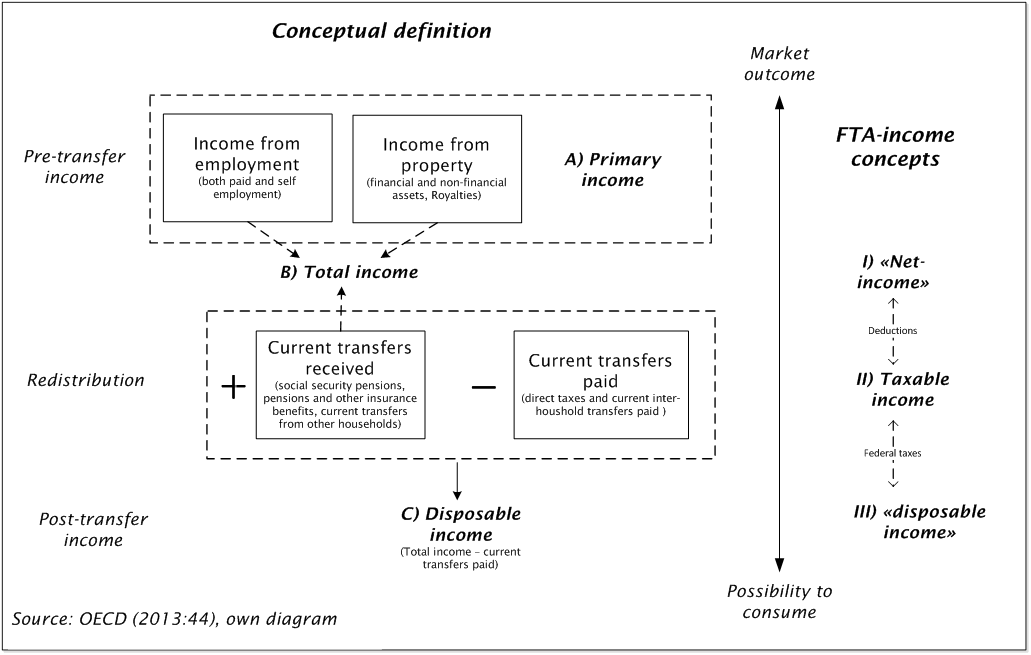
\includegraphics[width=\maxwidth]{figure/income_definition}
\caption{Income definitions}
\label{fig:incdef}
\end{figure}

% Quelle zu Abzügen:
% http://www.bilanz.ch/invest/steuern/netto-oder-reineinkommen
% Die rechte Seite mit den Steuergrössen könnte ausführlicher beschrieben werden
% Beispielsweise könnte man zeigen was Nettoeinkommen, Reineinkommen und steuerbares Einkommen sind
% Allerdings steht uns nur Reineinkommen und steuerbares Einkommen zur Verfügung

% ACHTUNG: Wir m?ssen innerhalb des Papers einheitlich bleiben. In der Grafik steht jetzt "Total income" oben steht "Net income"

% Man k?nnte es auch konzeptionell auf kantonale Steuerdaten erweitern. Besser w?re es, dies einfach im Ausblick zu erw?hnen

The central income reported through tax statistics is the taxable income. It includes all reported incomes (income from employment, income from property and received transfers\footnote{ Mean-tested benefits are not taxed and therefore not included in Tax data. Income for low income groups are therefore underestimated. However, Piketty and Saez (2001) note that non-taxable social security benefits grew as a share of personal income in the US but find that these changes had only a trivial impact on top income shares.}) minus several deductions. It is therefore neither a pre-transfer income  nor a post-transfer income measure. It's rather something in between. As the FTA tax statistics include some but not all deductions\footnote{The difference between the real Total income and the taxable income are deductions. This includes: professional expenses, travel expenses, interest on debt, Alimonies, Training costs, two-earner deduction, Party Contributions, Payment into pillar 3a, purchases in the pension fund and sideline deductions} it is possible to calculate a sort of "total income". As some deductions can be interpreted as compulsory expenses similar to taxes the step towards Total income is a step away from the income, which can be used for consumption. Similar when calculating the disposable income out of the taxable income through accounting the reported federal taxes, this is a step towards the income, which is left in the basket for consumption (disposable income). Again it is not a "pure" disposable income, because cantonal, municipal taxes and taxes from churches, which represent the bulk of taxes in Switzerland, are missing.   \\   

% Die Deductions sind noch nicht gänzlich sauber abgebildet. Auf der Bilanz-Seite steht, zum steuerbaren Einkommen kommt man, indem vom Reineinkommen die Sozialabzüge(Kinder- und Fremdbetreung) sowie der Abzug für unterstützungsbedürftige Personen abzogen werden. 
% Auf den ESTV-Tabellen sind jedoch noch mehr Abzüge abgebildet. Was soll/muss/können wir nun abziehen? Bin verwirrt...

% Allenfalls darauf hinweisen, dass die Wahl der Einkommensdefinition von der Forschungsfrage abhängt. Inequality in market outcome (genderdifferences) requieres to look at market earings from employment, to assess the role of redistribution different steps of income has to be looked at. Following the idea of economic wellbeing usual disposable income is looked at


\emph{statistical units} \\

The agreed standard on the statistical unit, which should be the base of inequality analysis, are households not individuals \citep[60]{oecd_oecd_2013 UNSICHER}. Indeed it are the individuals, who receive income, own wealth and experience economic wellbeing, but their possibility to do so, is strongly tied to the concept of household. This comprises all persons under the same housing arrangement. The basic underlying assumption for collection data on households level instead of individual level is, that people in the same household share resources and therefore pool their incomes (when two or more earners live together) and/or use the household income to provide the essentials of living for every household member (also non-earing members, like children). Additionally, there are economies of scale when people share living space and commodities and they therefore benefit from the sharing. The compare the individual economic well-being among individuals living in different households usually equivalence scales are used (see \citealt[173]{oecd_oecd_2013 UNSICHER}, \citealt{Buhmann et al., 1998 FEHLT}). \\

In tax data, however, the units are represented according to administrative rules. Tax units therefore neither represent individuals in every case nor true households. Tax units rather represent individuals and couples, but couples, who are married or officially registered. This doesn't imply, that those couples live together, as it is needed to satisfy the definition of a household. On the other hand, is it quit likely that more than one tax units live in the same household (unmarried/unregistered couples, see \citet[99]{muller_vermogenslage_2014}). It is therefore not directly possible to elicit households and household income out of tax data. This might influence the assessment inequality, taking into account the change from traditional household and family structures over the last century. 


% Allenfalls die Br?lhart-Daten erw?hnen und die m?glichkeit der Haushaltsbildung ?ber Abz?ge. Falls wir auch eine Grafik zur Rolle der Haushaltszusammensetzung machen (ich denke schon)
% gibt es studien? Zur Bedeutung von ?quivalenzskalen und zur Bedeutung der Differenzierung von Haushalten und Individuuen?
% inequality and family structure> review ny (McCall & Percheski (2010))
% Was ist zu erwarten, wenn Äquivalenzskalen vernachlässigt werden? Soll man dies erwähnen oder einfach weglassen

\emph{Measuring inequality or concentration} \\
To be able to make qualifying statements about a distribution or to compare different distributions, the concept of inequality turned out to be the most appropriate and thus the most commonly used dimension. The Gini coefficient is the most known measure and mainly used for international comparison. As it is derived from the lorenz-curve, the quantified amount of inequality can unpretentiously be described in a formal and visual way. Therefore the Gini coefficient is easely interpretable. Furthermore it has several desired statistical properties \citet{engelhardt_modelle_2000}. (1) principle of population: the assessment of inequality is independent of the population size (2) Bresciani-Turroni: the measure is sensitive for changes of income shares, but not for absolute changes (e.g. doubling of all income) (3) weak principle of transfers (pigou-dalton): transfers from richer households lead to a reduction of inequality. However, several drawbacks are reported in the literatur. The most important point is, that the underlying distributional form of the measured inequality is unknown and it is therefore not possibel to see if the measure is driven be a few rich or many poor individuals. This can also be problematic for comparision between countries or over time. In extreme cases two totally different distrubtions share the same gini-coefficient.\\

The recent wave of tax-data studies do not report Gini-coefficents. Rather top income shares are informed on, which are calculated not only with taxdata, but togehter with external sources to produce the population and personal income control totals. This procedure ensures, that the inequality measure is not biased because of non-fillers, who doesn't appear in tax statistics.  Leight (2002:594f) compares top income shares with other inequality measures and asks, if they are a useful measure of inequality in a society. He tries to answer this question empiricaly by comparing measures of inequality based on top income shares with measures of household or familiy inequality. He finds a strong positive relationship, but concludes (P.600): top income shares are far from perfect as a measure of distribution of income across society. Top income shares hence inform not completely on how inequality evolves elsewhere in the distribution. Furthermore, top income shares only weakly satisfy the Pigou-Dalton transfer principle (in contrast to the Gini-Coefficent see above). A transfer from rich to poor will indeed never increase the top income shares, but if the transfer is between invidviduals, who are either both within the top group or both outsie the top group, then the share measure will remain unchanged. \\

Newer branches of inequality studies emphasize the need for broader measures of inequality, which allow better analyses about the change of inequality and namely statements about the area of change (downgrading/upgrading). The polarityindex is developed by \citep{Handock and Morris 1999} allows for this. Recenently this index was applied in the work of \citep{Alderson, Beckfield and Nielsen 2005 FEHLT} and \citep{Alderson and Doran 2013 FEHLT}. This approach is rooted in relative distribution methods. It includes a precise comparison of the shape of two distributions (groups, over time). The main advantage lies herin, that this approche allows to characterize the change, in the sense that it is possible to say, if a polarization occured (reduction of middle class), which equals an increase of inequality and if this change is driven by a change in the upper or lower part of the distribution.  \\
 
The literature mentions several other metrics with desired properties, but we will not discuss them further (see for example \citet{cowell_chapter_2000} and \citet{hao_assessing_2010}).

% Allenfalls auch auf Quintilvergleiche eingehen und Atkinsonmass 


\emph{Population Coverage}
% beim letzten Punkt geht es um Steuerhinterziehung. Fällt das auch noch unter Population coverage?
 
Often inequality is assessed on national level, which implies, that studies try to cover the whole population of the country of interest. This is a special thorny task for surveys working with samples, because nonresponse is a major source of bias \citep{bethlehem_handbook_2011}.  \citep{korinek_survey_2006} show, that the position in the income distribution influence the probability to participate in a survey. Low income and high income households are more likely to refuse survey response, which leads to an overrepresentation of middle income households. This process can be referred to as the "middleclass bias" \citep{diekmann_empirische_2009}. Missing data in household surveys is therefore not missing at random, which has an impact on the measures of inequality. The magnitude of this bias in Switzerland, however, is unknown. Strategies to handle this kind of bias are discussed in the literature \citep{S?rndal et al. 1992 FEHLT}, but require a register for every unit, that is proportional to income. Currently there exists no such register for Switzerland \citep{ecoplan 2014:43 FEHLT}. Currently used micro datasets, which are used for official publications concerning inequality in Switzerland (SILC and HABE) are furthermore confronted with a constructed coverage problem, because these surveys rely on the phone register, which excludes the households not having a registered connection. \\
%(Problems of collective households, ecoplan 2014:45). Erw?hnen?

The issue of incomplete coverage is less dramatical with tax data. Essentially every permanent resident in Switzerland, who has completed the age of 18 years (respectively 20 years prior to 1996) is taxed on a yearly base (or every two years before the change of the tax system). Essentially this leads to a full representation of the adult population of Switzerland and a complete coverage of the income distribution. This includes a separation of normal cases, which embrace the majority of taxpayers, and the special cases, which cover Foreign nationals living in Switzerland but with a yearly or any other temporary resident permit only. Most important this includes high net wealth individuals taxed according to their expenditures. Special attention has to be paid to tax units with none or very low incomes. Even though they have to hand in a tax return, their income does not show up in the statistics if their income after deductions falls below 15'000 CHF and they are therefore not taxed with direct federal taxes. This is possible for normal and special cases alike. From 1995/1996 until 2010 the number of non-taxed units are reported, but not for the years before. Dell et al. (2007) try to estimate the fraction of non-taxed by comparing the reported numbers of tax units to census reports about the number of adult population. Following his etimations this fraction drops from 94\% in 1993/1994 to 63\% back in 1945/46. \\

An other critical issue with tax data is the problem of tax evasion, which definitely can bias the assessment of inequality. Alvaredo and Saez (2006) for example regard estimates of Spanish top incomes prior to 1981 as unreliable due to widespread tax evasion. Evasion can occured, when individuals try not to fill tax returns or by misreporting of incomes. In Switzerland non-fillers show up in the tax-statistics either way, as long as they are registered. This person get an imputed income form an older tax return and infomration given by employers. Only non registered non-fillers are not in the records. Therefore non-fillers are a minor problem. Not neglectable is the circumstance, that individuals misreport incomes. \citet{feld_tax_2006} examine the role of tax evasion in Switzerland by calculating the difference of the national accounts measures of primary income and the income reported to the tax authorities. They can show, that the average level of income tax evasion from 1965 to 1995 varies between 13\% and 35\%. They suggest, that evasion is heavily driven by capital income tax evasion. \\




\emph{Intertemporal comparison}

One advantage of tax data over survey data is their observation period. While the FTA data we use range back to 1945, the earliest period of survey data is 2000 (HABE data). To be fair, survey data might cover the late periods (2011 and 2012) which are not covered by tax data. The striking feature of the long FTA time series is its consistency. Both population coverage and income measures are consistent for the complete observation period. This can not be said for survey data as these are based on samples and therefore require an ideal sampling design or reweighting to be representative and comparable over time. We will see how well sampling and weighting is done in the results section.

\subsection{Comparison of tax data and other data sources - advantages and shortcomings}

% Suitability of data sources can be judeged by different criterias. crossectional or longidutional perspective. longidutional perspective allows for dynamic 

%[ich stelle mir eine Tabelle mit verschiedenen Dimensionen vor, anhand derer eine Einordnung unterschiedlicher Datenquellen geschieht.]
% Mögliche Vergleichsdimensionen
%- Suitability of cross country comparison
%- Coverage of the population of interesst
%- Implementation of common concepts of economic ressources
%- intertemporal comparision
%- flexibel applications of appropriate inequality measures
% - appropriate income definition

\begin{table}[h]
\begin{tabular}{lcccc}
                                   & FTA       & HABE      & EU-SILC   & LIS       \\
Range                              & 1945-2010 & 2000-2011 & 2007-2012 & 1982-2004 \\
Cross country comparison possible? & no        & no        & yes       & yes       \\
Top incomes covered?               & yes       & no        & no        & no        \\
Low incomes covered?               & no        & yes       & yes       & yes       \\
Concepts of economic ressources?   & no        & yes       & ?         & ?         \\
Equivalisation?                    & no        & yes       & ?         &          
\end{tabular}
\end{table}

% Braucht es alle drei Survey-Befragungen
% ich würde nicht dichotomisieren, sondern ordinal bewerten (tief, mittel, hoch)

% Die Punkte kurz beschreiben.
% Zusammenfassung


% Gedankenstütze
%\textbf{Problems with household income surveys}
%\begin{itemize}
%\item Sample data (bias)
%\item comparability between countries and over time (depends on income definition)
%\item short time series
%\end{itemize}


%Burkhauser et al. (2009) compare inequality statistics form survey data and tax records to consolidate the findings about recent trends in the USA
%Studies on problems with survey data See for other countries: \citealt{Siminski et al 2003 FEHLT} (Australia), \citealt{Brewer et al 2008 FEHLT}, UK, \citealt{Burkhauser et al. 2009 FEHLT}, US)


%Warnings about the use of tax data
%The use of tax data is often regarded by economists with considerable disbelief. These doubts are well justified for at least two reasons. The first is that tax data are collected as part of an administrative process, which is not tailored to the scientists' needs, so that the definition of income, income unit, etc., are not necessarily those that we would have chosen. This causes particular difficulties for comparisons across countries, but also for time-series analysis where there have been substantial changes in the tax system, such as the moves to and from the joint taxation of couples. Secondly, it is obvious that those paying tax have a financial incentive to present their affairs in a way that reduces tax liabilities. There is tax avoidance and tax evasion. The rich, in particular, have a strong incentive to understate their taxable incomes. Those with wealth take steps to ensure that the return comes in the form of asset appreciation, typically taxed at lower rates or not at all. Those with high salaries seek to ensure that part of their remuneration comes in forms, such as fringe benefits or stock-options which receive favorable tax treatment. Both groups may make use of tax havens that allow income to be moved beyond the reach of the national tax net. These shortcomings limit what can be said from tax data, but this does not mean that the data are worthless. Like all economic data, they measure with error the 'true' variable in which we are interested.
%The data series presented here are fairly homogenous across countries, annual, long-run, and broken down by income source for several cases. Users should be aware also about their limitations. Firstly, the series measure only top income shares and hence are silent on how inequality evolves elsewhere in the distribution [why?]. Secondly, the series are largely concerned with gross incomes before tax. Thirdly, the definition of income and the unit of observation (the individual vs. the family) vary across countries making comparability of levels across countries more difficult. Even within a country, there are breaks in comparability that arise because of changes in tax legislation affecting the definition of income, although most studies try to correct for such changes to create homogenous series. Finally and perhaps most important, the series might be biased because of tax avoidance and tax evasion. For the details, we refer users to the original papers (see also Atkinson, Piketty and Saez, 2011).



\subsection{Outline of applied methods}

% Diese Abschnitt muss ersetzt werden mit der von uns gewählten Vorgehensweise

In the last section we described the advantages and drawback of taxdata discussing five aspects, which we regard as crucial concering the assessment of inequality. To get a feeling of the importance of these aspects, we exploit the FTA-tax data as far as possible and perform several insightful calculations adressing four of the five mentioned aspects. No further investigation is possible regarding aspect (1) concepts on measuring economic ressource. This is a point which cannot be further addresses with FTA tax data. But for the other four thematic areas, we can provide deeper insight. In general our main strategy is to apply different possible concepts within one conceptional area (income, units, measurement, population coverage) while holding other conceptual differences constant. With this strategy we want to show, the sensitiveness the assessement of inequality is especially if one looks at time trens.  In this section we  describe which methods we use to produce the results in the next section.

%%%
% Was soll hier beschrieben werden und was direkt bei den Tabellen?
%%% Gar nicht so einfach....

%%% Nach Lehrbuch müssten die methodischen Schritte hier beschrieben werden.
% Man könnte zu den Zeitreihen jeweils die Varianz ausweisen-> dass würde helfen die Reihe zu beurteilen. Man sieht dann: aha, die Reihe ist im Vergleich zur anderen höher/tiefer. Ob die Reihen stärkeren Schwankungen unterliegen könnte einfach aus der Varianz gelesen werden


% Defining income
% Beschreiben, dass sich aus den publizierten Einkommensgrössen und den Steuerbeträgen unterschiedliche 
% Einkommen berechnen lassen
% Es steht der Vorwurf im Raum, die unteren Einkommen seien mit Steuerstatistiken schlecht abgebildet, weil bedarfsabhängige Leistungen nicht versteuert sind

% Es müsste eine Reihe zum gesetzliche Grundbedarf vorliegen. Wüsste ich jetzt grad nicht von wo...

%%
% statistical units
% Beschreiben, dass zwar keine Haushaltseinkommen gebildet werden können und Skaleneffekte nicht abgebildet sind, dass eine Annäherung jedoch möglich ist
% Definition der äquivalenzskala bei Brülhart (korrespondiert nicht mit OECD Definitionen, aus pragmatischen Gründen)

%%
% Measuring inequality
% Beschreiben, wie sich aus gruppierten Steuerstatistiken der Gini-Koeffizient berechnen lässt
% Beschreiben wie wir relative distribution technics einsetzen und den Polaritätsindex berechnen

% Calculate the gini
% Ein bisschen erklären, wie aus gruppierten Tabellen der Gini-Koeffizient berechnet wird.

% Polaritätsindex
% Alderson and Doran (2013:56) beschreiben zwei mögliche Indizies Median relative polarization index (MRP) eingeführt von (Morris, Bernhardt und Handcock 1994:217), der in den lower relative polarization index(LRP) und den upper relative polarization index (URP) zerlegt werden kann (ebd.209)
% (1. Schritt) Probability density functions
% (2. Schritt) Overall relative density function -> Achtung diese Dichtefunktion bildet sowohl die  Lokationsverschiebung als auch durch Verschiebung der Form ab. Eigentlich interessiert aber, der shape shift
% Deshalb wird die Verteilung um die Lokationsverschiebung bereinigt und nur der shape-shift angeschaut. Ausgewiesen werden (MRP)-> hat polarisierung stattgefunden: LRP und URP-> ist polarisierung eher auf eine Zunahme armer (LRP) zurückzuführen oder auf eine Zunahme von Reichen? (URP)


%%
% Population coverage
% Analysen zu den Nullern > ist eine Hauptkritik an der Nutzung von Steuerdaten
% Die Bedeutung von Normal- und Sonderfällen
% Den Vergleich mit der HABE beschreiben, welche Einkommensgrösse nutzen wir aus der HABE um diese möglichst mit den Steuerdaten vergleichbar zu machen? Wir brauchen das Bruttoeinkommen nach Abzug der Sozialversicherungsbeiträge, dies lässt sich mit dem Reineinkommen vergleichen




%%
% Intertemporal comparison
% Ziel eine möglichst lange Zeitreihe abzubilden. 
% Technik der Lückenfüllung von Ben beschreiben> dies kurz anderen Techniken gegenüberstellen.
% Konfidenzintervalle für die Perioden mit vielen fehlenden Werte?

% eine / oder zwei Zeitreihen (eine lange und eine, die möglichst nahe an der richtigen Konzeptionalisierung ist: post direct taxed income, normal+sonderfälle) zusammen mit den bereits existierenden Reihen (HABE,LIS,SILC) ploten



\textbf{Incomplete coverage of the population (left censored data.)} What can be done about the not-taxed? \citet{dell_income_2007} impute for non-fillers the 20 percentage of the annual average income. This flattens the distribution on the left side, which is not a problem if you are interested in the top income shares, but it would surly affect overall measures of inequality. Furthermore the authors calculate the proportion of non-fillers by estimating the total of tax units out of the population records. \\

\textbf{changes in taxation system  (switch from annual to biannual taxation)} In the mid-1990s a fundamental change in the Swiss tax system took place by switching form the two-years based praenumerando taxation to the one-year based postnumerando taxation. This change was enacted with a transitional period of several years, during which each canton could choose when to adopt the new system.  This is why during the transitional period from 1995 to 2003 there is no uniform tax data published on the Swiss level but only data on the cantonal level \citep[8f]{foellmi_volatile_2013}. \\
%es wird erwartet, dass der Wechsel Ungleichheitsmasse beeinflussen. Yearly fluctuations are dampened, when income is measured on a two-yearly basis.

\textbf{Estimating percentiles from bracket income tabulation} Pareto interpolation \\ 

\textbf{Missing of mean-tested benefits as part of the income} -> imputation with recommendation for minimum level for basic needs defined by the SKOS.\\
%is never mentioned as a problem, but it seems to me a better way to approach the non-taxed issue, than dell way (20 % of average income)
% Beim Imputieren m?sste man auch die Zahl der freiwilligen Nichtbeziehenden ber?cksichtigen.

\textbf{deductions} \citet[477]{dell_income_2007}:" we can check with statistics for 1971-72 (as well as later years) presented both by size of income before deductions and income after deductions that adding back deductions does not introduce any significant error in our estimates."
\citet[5]{schaltegger_evolution_2011 UNSICHER}: ``..., information on [...] deductions is provided in the tax statistics, thus, we could add the personal deductions to the income data to obtain a consistent series over time''. Können wir das auch? Zumindest für gewisse Zeiträume? Das wäre noch gut. \\

Studies on income try to focus on the disposable income, which subtracts certain expenditures from the primary income. Deductions reflect somehow compulsory expenditures and thus taxable income can be seen as a sort of pseudo disposable income. On the other hand deductions can affect the distribution. There are recent studies about the correlation of progressivity and deductions in Switzerland, which examines if deductions have a ``perverse redistribution'' effect by redistributing income from the lower middle class to the upper middle class (see \citealt{peters_steuerabzuge:_2011} and \citet{Interpellation Barbara Gysel (2009) FEHLT. das interpellation barbara sieht falsch aus}.

% Income share specific problems
% Total income denominator Exogenous Approach -> net income reported in the national accounts. Endogenous Approach -> Dell et al. technic-> imputing 20\% of average personal income to non-fillers (which are mainly persons with low or no income). Honestly , is this appropriate? (Everyone did it)
% Total of tax units in the country. exogenous approach -> construct number of total tax units artificially from other data sources
% Endogenous approach -> reported in the tax tables 

%%%-------------------------------------------------%%%
%%% Abschnitte aus ersten Version des Papers %%%
%%%-------------------------------------------------%%%

%\subsection{Hypotheses}
%Based on the theories we test the following hypotheses:

%\begin{itemize}
%\item H1: Develpment of inequality is driven by sectoral change
%\item H2: Development of inequality is driven by political change, i.e. economic crisis contribute to inequality because welfare states tend to be downsized
%\end{itemize}

%\subsection{Data and Variables}

%We use data from the Swiss Federat Tax Administration (FTA) where our data about incomes ranges from the years 1941/42 to 2010. While the data results in a long and consistent time series to illustrate swiss inequality development, there are a few pitfalls we want to adress which might be of interest for other research on this topic (be it in Switzerland or other countries).

%\subsubsection{Left censored data}

%The FTA provides data about all tax units in Switzerland that are liable to pay federal taxes.A tax unit may be a single person or a household. The taxable population however is not identical to the population which should be used to calculate measures of inequality. Precisely, the data do not contain tax units with very little incomes so calculations based on these data treat the lowest percentiles equally to tax units with zero income.Figure X shows the threshold to be hit to enter the statistic.

%\textcolor{red}{[FIGURE X ABOUT HERE] soll zeigen: Zeitreihe der Untergrenze von 1941-2010}

%So first of all, there is a bias in the level of an inequality measure one could calculate with the   FTA data. Furthermore, also the changes over time might not be interpreted savely as over time the number of tax unit within this "hidden range" might vary or might even have a certain trend. We will adress this issue in detail in the methods chapter.

%\subsubsection{Different measures, different populations}

%The FTA data makes two kinds of distinctions. First, data was collected for so called "normal cases" and "special cases", i.e. a "normal case" is a taxable (for the complete tax period) person or household domiciled in a swiss canton without income from outside of Switzerland. A "special case" therefore is a diffuse reference category that contains tax units that are taxed at source, were not taxable for the complete tax period or generated additional income in another country. Second, the FTA reports two measures, that is taxable income and absolute income \textcolor{red}{(meine vorläufige Übersetzung von Reineinkommen)}. Absolute income is the sum of all incomes (earnings, interest income, rental incomes) minus expenses (e.g. from self-employment or credit cost). The taxable income is calculated as the difference of absolute income and deductions (e.g. children, insurance rates). The longest consistent time series exists for the taxable income of normal cases. So all statements we make with our data only apply to this subpopulation.

%\subsubsection{Changes in taxation and measurement}
%The swiss tax system is highly federal. That means, communities raise taxes which then go to the communities, the canton and the state. If we want to calculate overall swiss measures, we need to take into account, that cantons vary (between cantons and over time) with regard to the tax deductions that are possible and also the mechanism how taxes are collected. The latter adresses a comprehensive reorganization of the swiss tax system where between 1995 and 2003 cantons changed from taxing the past two years of income (postnumerando system) to taxing the present single year (praenumerando system). For details see \textcolor{red}{Martinez (xxxx) or some other author (xxxx)}. Aggregate measures of inequality therefore have to be estimated for the periods 1995 to 2003 which we adress shortly in the methods chapter.

%\subsection{Methodology Used}
%There are two steps of data analyses which need to be described to the reader. First, the estimation of the bias we introduce by estimating measures of inequality when tax units with too little income are not observed. Second, the steps undertaken to estimate aggregate swiss measures by imputing taxable income for those cantons and periods where the change of the tax system produced a gap (1995 to 2003, depending on the canton). 

%\subsubsection{Imputing the gap}
%The imputation is not a focus of the paper so we basically follow the most simple approach of Martinez (xxxx). That is estimating the missing taxable income statistics via OLS using information from time trends and cantons. Our imputation model therefore includes canton inequality measures and periods dummies to explain aggregate swiss inequality.

\subsubsection{Estimating the bias}
For most of the observed range (1941 to 2010) we do not have any information how many tax units fall into the category of having income that is not zero but is too little to qualify for federal taxation (lets call those ``zeros'' for convenience) . However starting 1995, the FTA provides exactly this information for each canton. This enables us to estimate the bias we introduce for each canton and each period between 1995 and 2010. Consequently we can obtain information whether the bias is stable over time (which makes it possible to safely interpret the changes of inequality over time) and whether the bias is different for each canton. \textcolor{red}{Unterschiede zwischen Kantonen wären gut um zu argumentieren, dass andere Länder auch davon betroffen sind, in etwa sowas wie ``je höher der Steuerfreibetrag, umso stärker der Bias''. Länder de erst sehr spät besteuern (und über nicht Besteuerte dann auch nicht Buch führen) haben einen krassen Bias. Wir könnten dann empfehlungen geben, ab welchem Perzentil man save interpretieren kann oder so.}

One can take a first look at the descriptives plotting the share of zeros over time seperately for each canton.




\begin{knitrout}
\definecolor{shadecolor}{rgb}{0.969, 0.969, 0.969}\color{fgcolor}
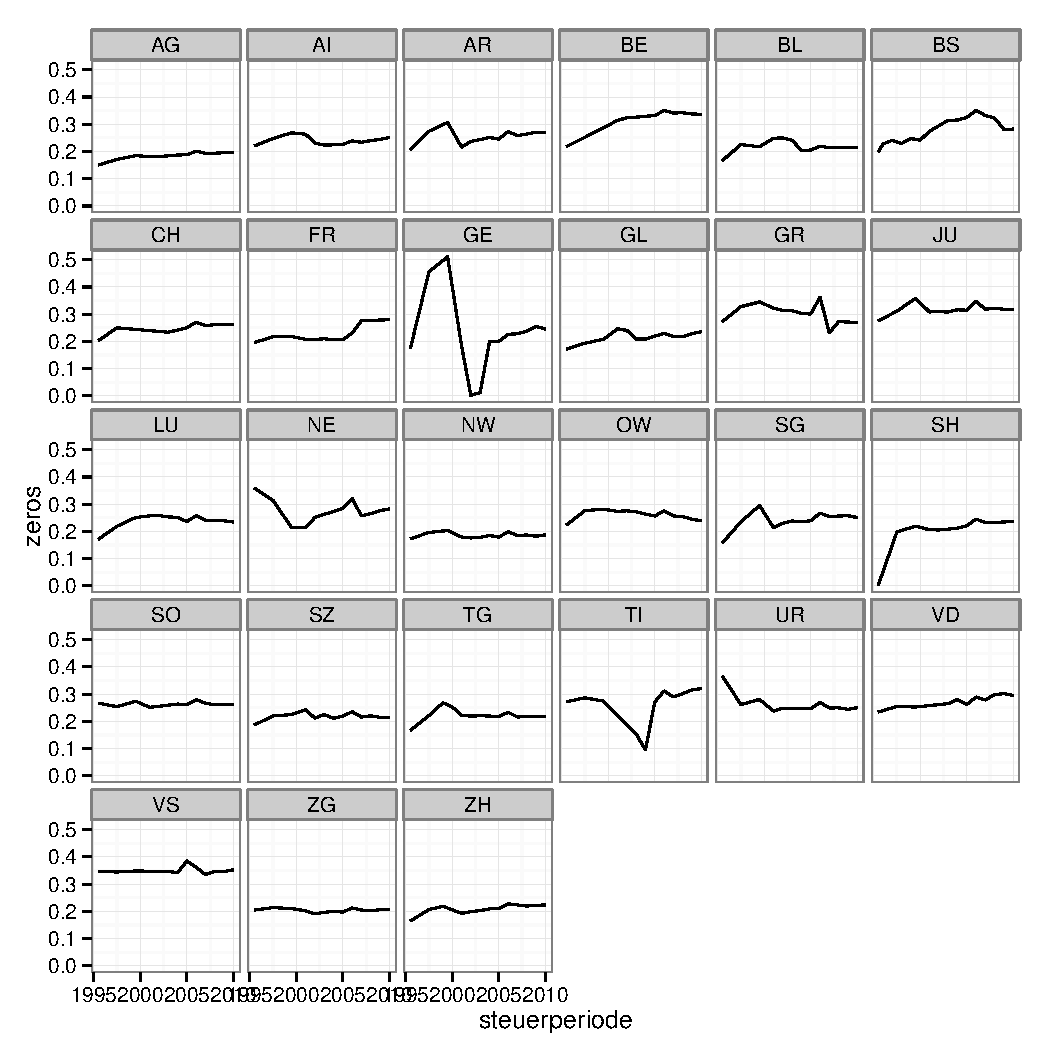
\includegraphics[width=\maxwidth]{figure/zero_descriptives1} 

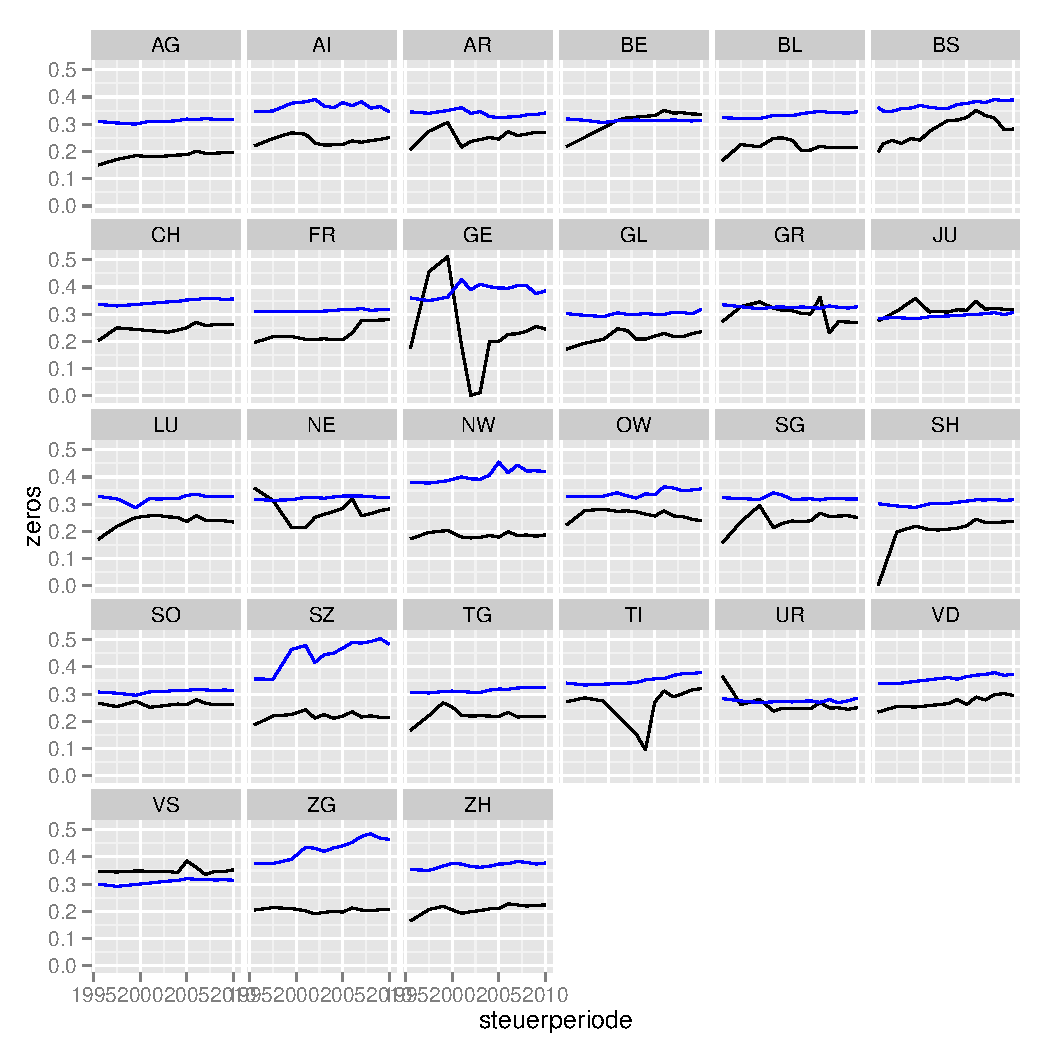
\includegraphics[width=\maxwidth]{figure/zero_descriptives2} 

\end{knitrout}


We can see multiple things here:

\begin{enumerate}
\item There is a small overall upward trend which we assume to be the Federal Administrations inflation adjustments to the tax threshold.
\item Geneva and Tessin show wild changes but those might be explained by the tax gap ("Bemessungslücke") that people exploited when the cantons changed the tax system. It remains unclear however why we can't see similar patter within other cantons.
\item There is some variance and we see different patterns over time and cantons. When estimating Gini coefficients or the like we must therefore assume that ignoring ``the zeros'' leads to a bias that is not stable over time.
\end{enumerate}

We might try two strategies to moderate the problem:

\begin{enumerate}
\item Add the zeros as a separate group
\item Fit a model to predict the inequality measure (e.g. the Gini coefficient) using the share of zeros as a predictor
\end{enumerate}

By adding the zeros as a separate group we face several problems. With the exception of Geneva 1995/96 Pareto interpolation of percentiles p20 and above seems viable. Low percentiles however would need to be extrapolated so we might impose unrealistic assumptions. Even when estimating ``safe'' measures above p20 (better p50) or a Gini coefficient we need to make an assumption about the income structure of that group (a distribution, a mean income or zero-income). To be consistent with the measure of ``taxable income'' we could assume an income of zero for that group, calculate Gini coefficients and compare them with the original (uncorrected/plain) version. To get a rough number we could (by cantons) check the squared correlation between plain and corrected Gini.

The second approach however is more robust as we do not impose additional assumptions but instead exercise some curve fitting.

\begin{knitrout}
\definecolor{shadecolor}{rgb}{0.969, 0.969, 0.969}\color{fgcolor}
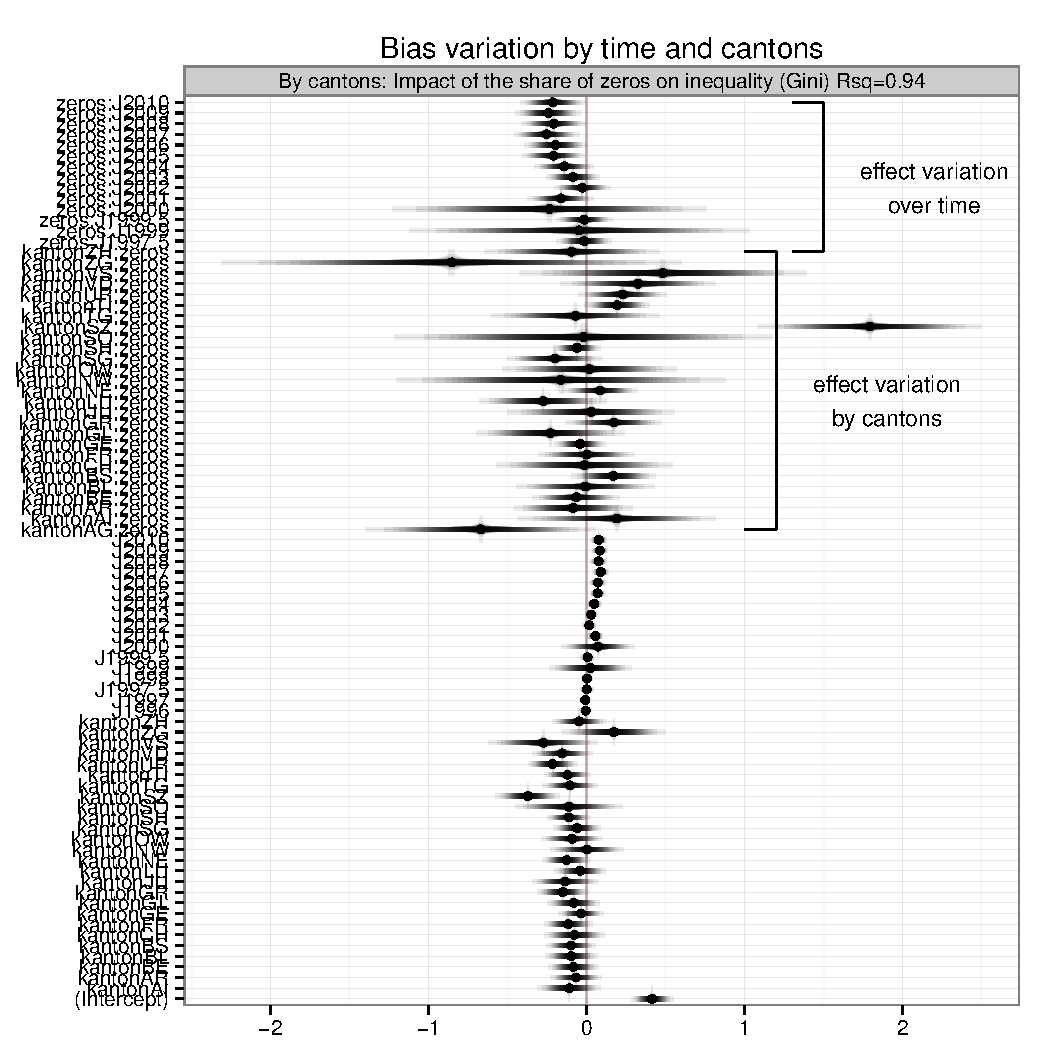
\includegraphics[width=\maxwidth]{figure/corrected_gini} 

\end{knitrout}


The model outputs a test statisic for each canton that tells us whether the variation of the zero-rate over time leads to a significant deviation from the typical ``canton gini-level''. As the model has a decent fit we are not in great danger of omitted variable bias. Using a joint F-Test we can now test if all canton interactions are zero. 




In our case we can clearly reject the hypothesis that all interactions are zero ($p=0$). This leads to the conclusion  that Gini coefficients are biased by the variation of the zero-share which is kind of obvious but at the same time we can use the model to report adjusted Gini coefficients. For example one might be interested in how inequality would had developed if the zero-share would have been constant over time. (Note RF: predict all data point using canton, time and the initial OR final zero-share to homogenize the time series)
Furthermore we can quantify how large the bias is and we can do this separately for tax periods or separately for cantons. 

For all cantons:




We can see the the model fit reduces to explaining 61.5\% of the Gini variation versus 92.6\% when the information from the zero-shares was used. Although this so some extent attributable to the additional 26 parameters: this is huge. 

The model indicates some cases that deserve more attention: Schwyz (positive coefficient) and Geneva (negative coefficient) and the tax period 2000 as well as the most recent periods.

A positive coefficient (e.g. Schwyz) can be read as follows: In periods with many zeros we measure higher Gini coefficients. We can derive, that the distribution of income is more skewed for high incomes than for low incomes. Simply speaking, the contrast between low and middle class is less pronounced than the contrast between middle and top class. One possible explanation would be that incomes stem from two different populations: 1) the people of Schwyz who possibly follow a log-normal or gamma distribution and 2) particularly rich people who moved to Schwyz to avoid taxes. 

A negative coefficient (e.g. Geneva) means the more zeros there are the smaller the Gini measure was compared to other tax periods within that canton (remember this is a fixed-effects model). This is the case we would usually expect: more zeros mask inequality that arises from the bottom.

What can we conclude from that analysis? First one must notice that aggregate measure like the Gini (or others) do not always react in the same way when we cut off one part of the distribution, therefore the measures calculated from tax data is biased. On the other hand, the model coefficient of Switzerland as a whole is not significant suggesting that the cantonal biases cancel out each other. This seems plausible. Most of the ``tax optimization'' happens within Switzerland so the rich people who moved to Schwyz are now missing at another canton.

We can even see more from the model coefficients. The period dummies indicate how the distribution of incomes has changed: compared to 1995, the subsequent periods have a negative coefficient, i.e. the bias we introduce by omitting the zeros increased, especially from the mid nineties to the mid 2000s. To simplify: cutting off zeros more and more seems to lead to an underestimation of our inequality measure, probably because the skewness in the left part of the distribution increased pointing to an increased pauperization that is masked by omitting the left tail of the income distribution.




% Alter Textbaustein zu Vermögen
%\emph{Defining wealth}
%While the apropiateness of the conceptualization of income is widely discuded, there is no agreed definition of personal wealth yet and the appropriate methods of valuation are not always clear. Wealth can be defined as the marketable value of financial assets plus non-financial assets (housing and land) less debts (Credit Suisse 2011:5).

%The discussion about problems with reporting income is fairly exhaustive. What about wealth?

%It is well recognized that the traditional sources of wealth distribution data are unlikely to provide an accurate picture of wealth ownership in the top-tail of the distribution. \citet{credit_suisse_global_2011} makes use of the information in the ``Rich Lists'' published by Forbes Magazine to adjust the wealth distribution pattern in the highest wealth ranges. \\

%Additionally the Credit Suisse Reports states that these data my be less subject to response bias, but my be more prone to valuation problems, especially in connection with pension assets and debts \citep[8]{credit_suisse_global_2011}.





%%%-------------------------------------------------%%%
%%% Include results %%%
%%%-------------------------------------------------%%%


%%%-------------------------------------------------%%%
%%% Sub document results %%%
%%%-------------------------------------------------%%%

\section{Results}

% Brauchen wir glaubs nicht mehr
%\textcolor{red}{Gesamtschweizer Grafik (mit imputierten Daten) einmal eine Linie mit Bias, einmal ohne
%Kantonsweise Grafiken
%Kuznets / U-Turn, Test der Hypothesen mit den final Daten. Der link zwischen rein deskriptiv  und Theorie plus Modell ist aktuell noch ein krasser Drahtseilakt...}

% Der Übersicht halber habe ich hier die Titel hier analog zum "Struktur-Issue" auf git gesetzt

\subsection{Defining income}


\emph{Gini coefficients for taxable income, income before deductions and taxable income after tax}




\begin{knitrout}
\definecolor{shadecolor}{rgb}{0.969, 0.969, 0.969}\color{fgcolor}\begin{kframe}


{\ttfamily\noindent\itshape\color{messagecolor}{\#\# \\\#\# Attaching package: 'reshape'\\\#\# \\\#\# Die folgenden Objekte sind maskiert from 'package:plyr':\\\#\# \\\#\#\ \ \ \  rename, round\_any}}\end{kframe}
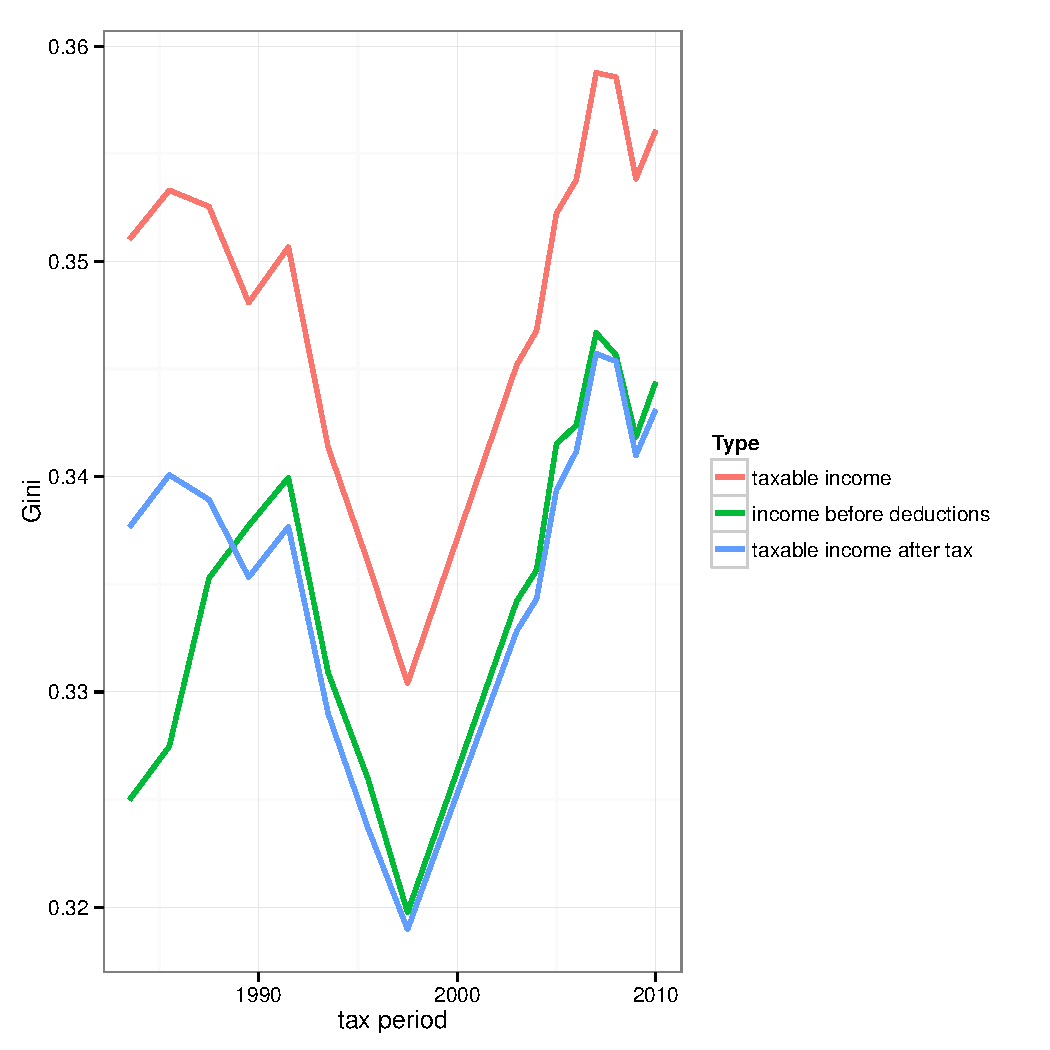
\includegraphics[width=\maxwidth]{figure/different_ginis1} 

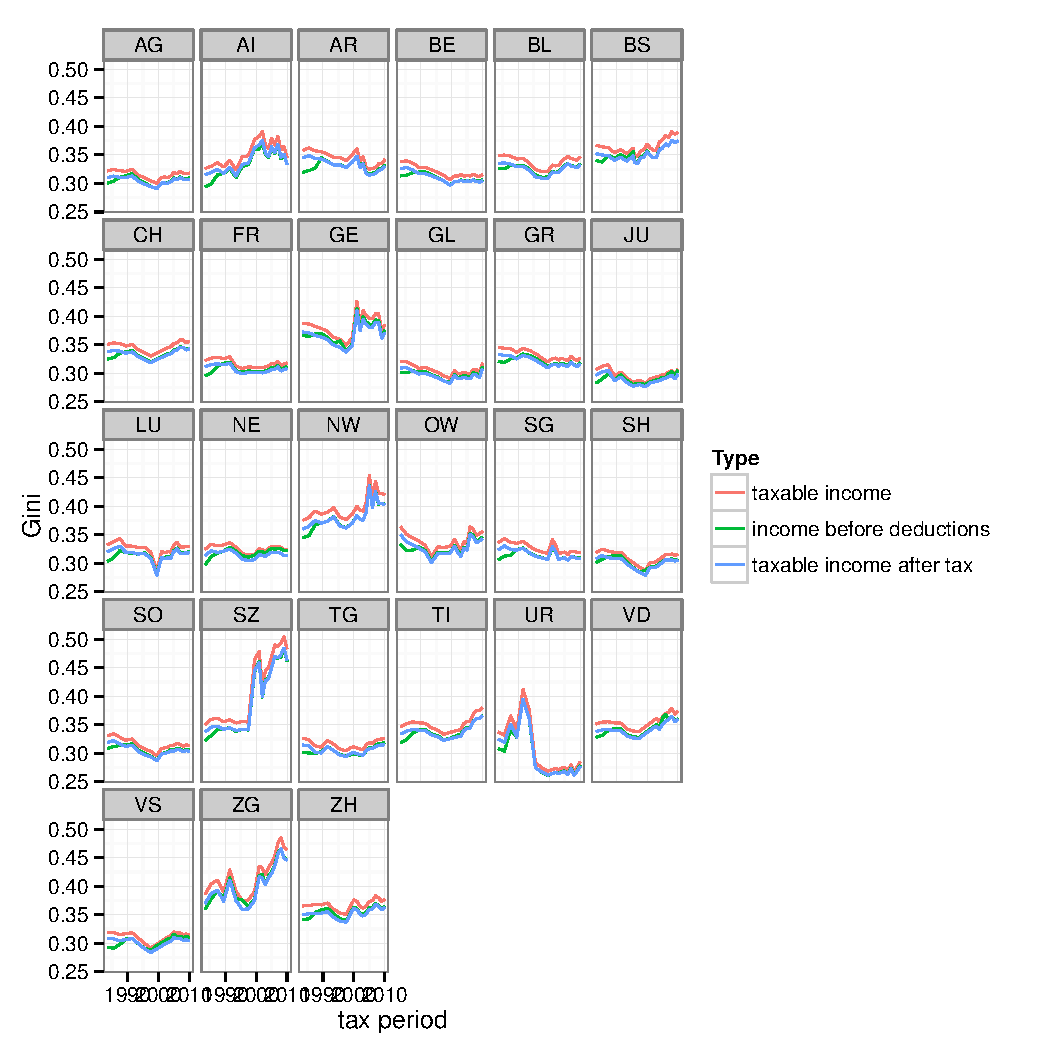
\includegraphics[width=\maxwidth]{figure/different_ginis2} 

\end{knitrout}



\emph{Gini coefficients considering mean-tested benefits}

\subsection{Measuring inequality}

% Zero-shares (alter Textbaustein)
%Estimation using population statistics (1945/46-1993/94) and official tax administration statistics (1995/96 and later) 
% Das allenfalls in der Methodensection machen?
% Vergleich mit der Dell-Reihe zu Non-fillers
% Überschneidungen gib es leider nicht 
% Interessant wäre es auch, zu sehen ob es Brüche in den Zeitreihen der Zahl der Steuerpflichtigen und jener ohne Besteuerung gibt.

\subsection{Population coverage}

\subsubsection{Normal versus special cases}

The FTA stopped to publicly report data for special cases after tax period 1993/94. 
For more recent periods however we can compare data from the 
BRUELHARTPROJEKT (wie nennen wir das?) to the FTA normal cases, as these data are 
identical but the BRÜLHART data include special cases. 
We will have a look at both, the 1993/94 period as the last period where both 
numbers were reported as well as 2009 where we compare data from the same source 
but using differnt data sheets.


%ABBILDUNGEN ZUM VERGLEICH NORMAL-/SONDERFÄLLE
\begin{knitrout}
\definecolor{shadecolor}{rgb}{0.969, 0.969, 0.969}\color{fgcolor}
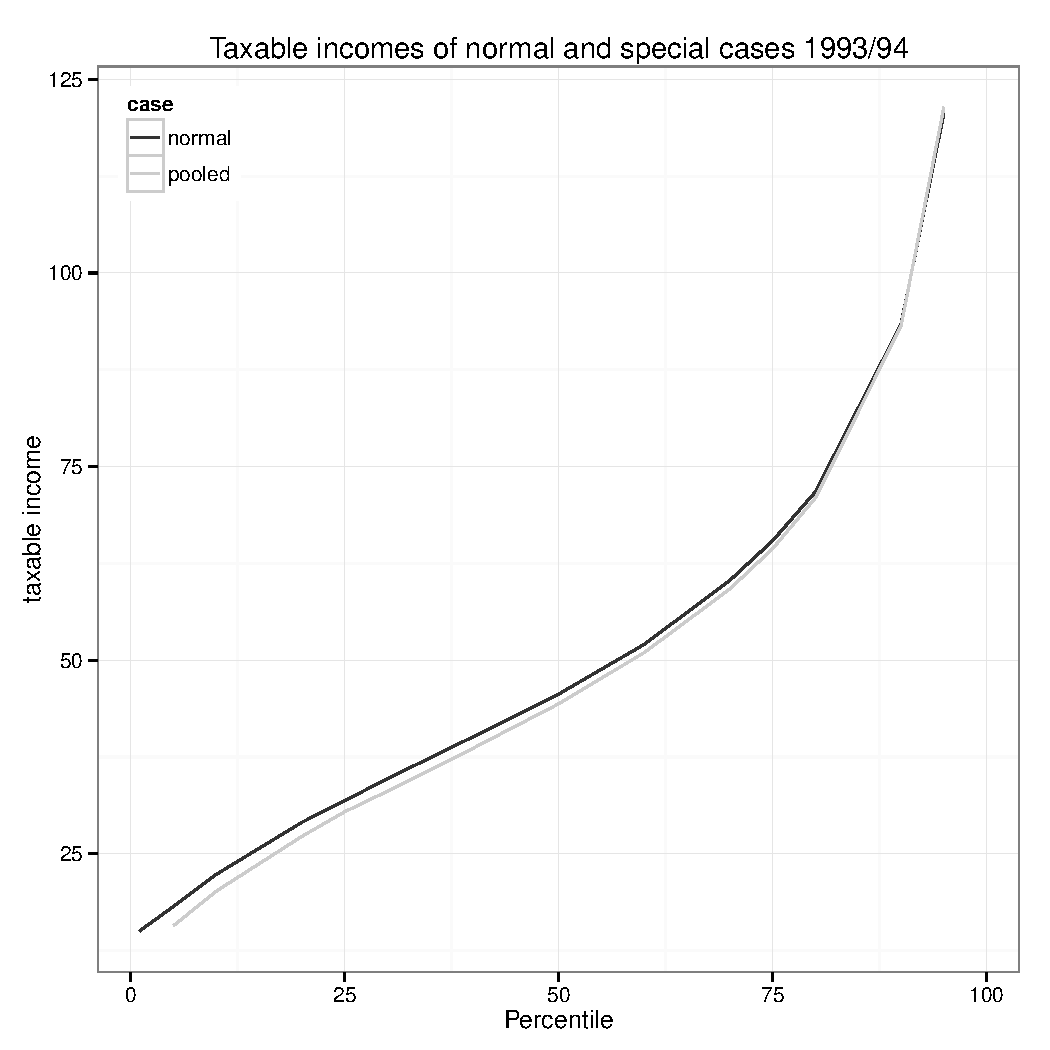
\includegraphics[width=\maxwidth]{figure/specialcases93941} 

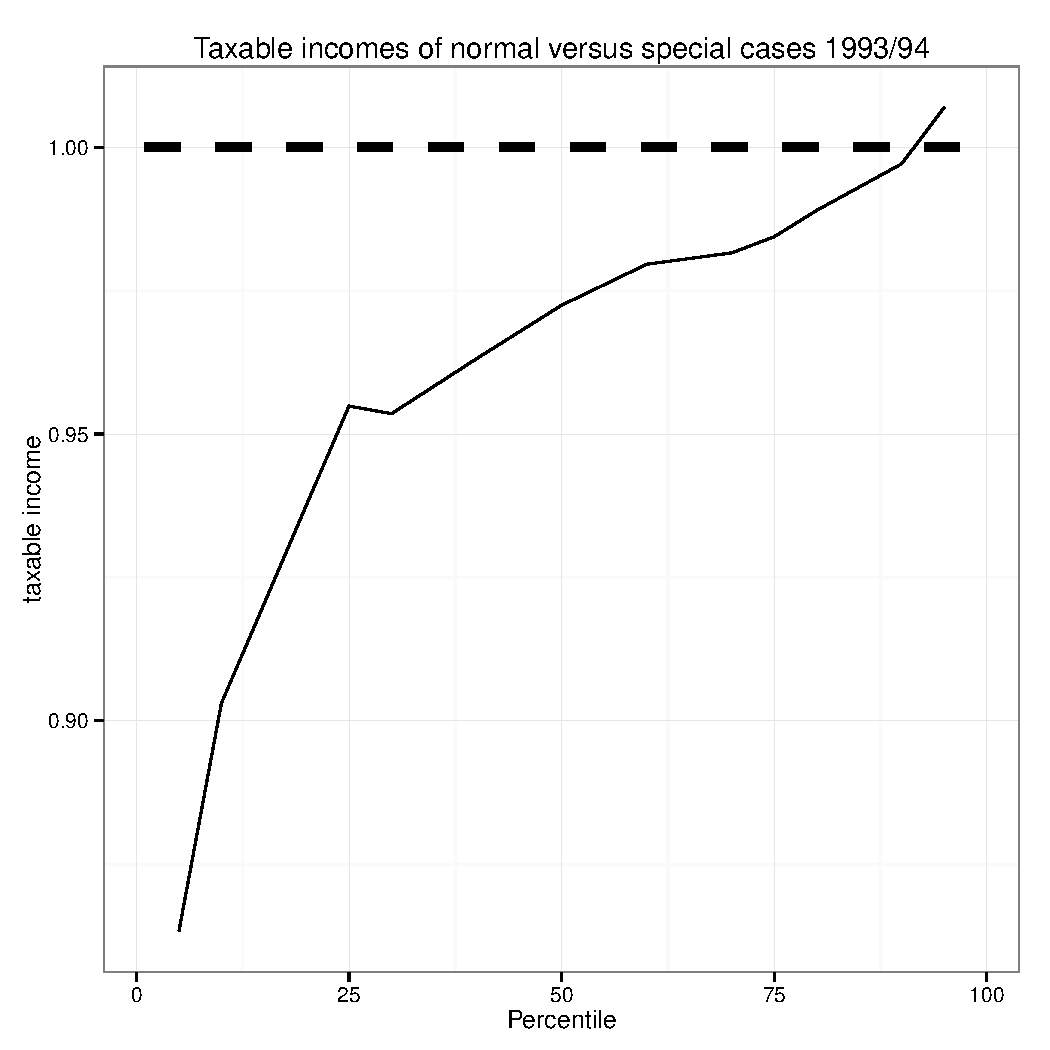
\includegraphics[width=\maxwidth]{figure/specialcases93942} 

\end{knitrout}


\begin{knitrout}
\definecolor{shadecolor}{rgb}{0.969, 0.969, 0.969}\color{fgcolor}
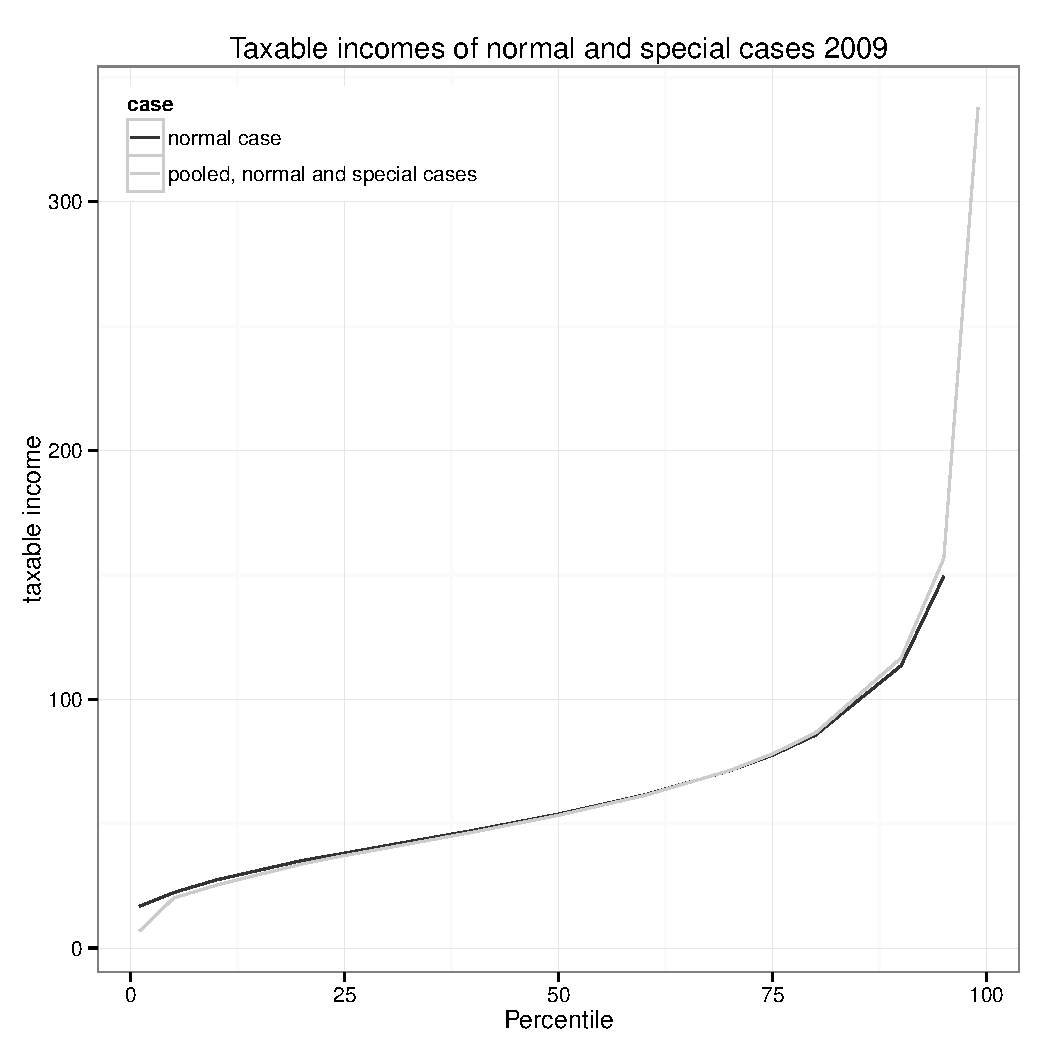
\includegraphics[width=\maxwidth]{figure/specialcases091} 

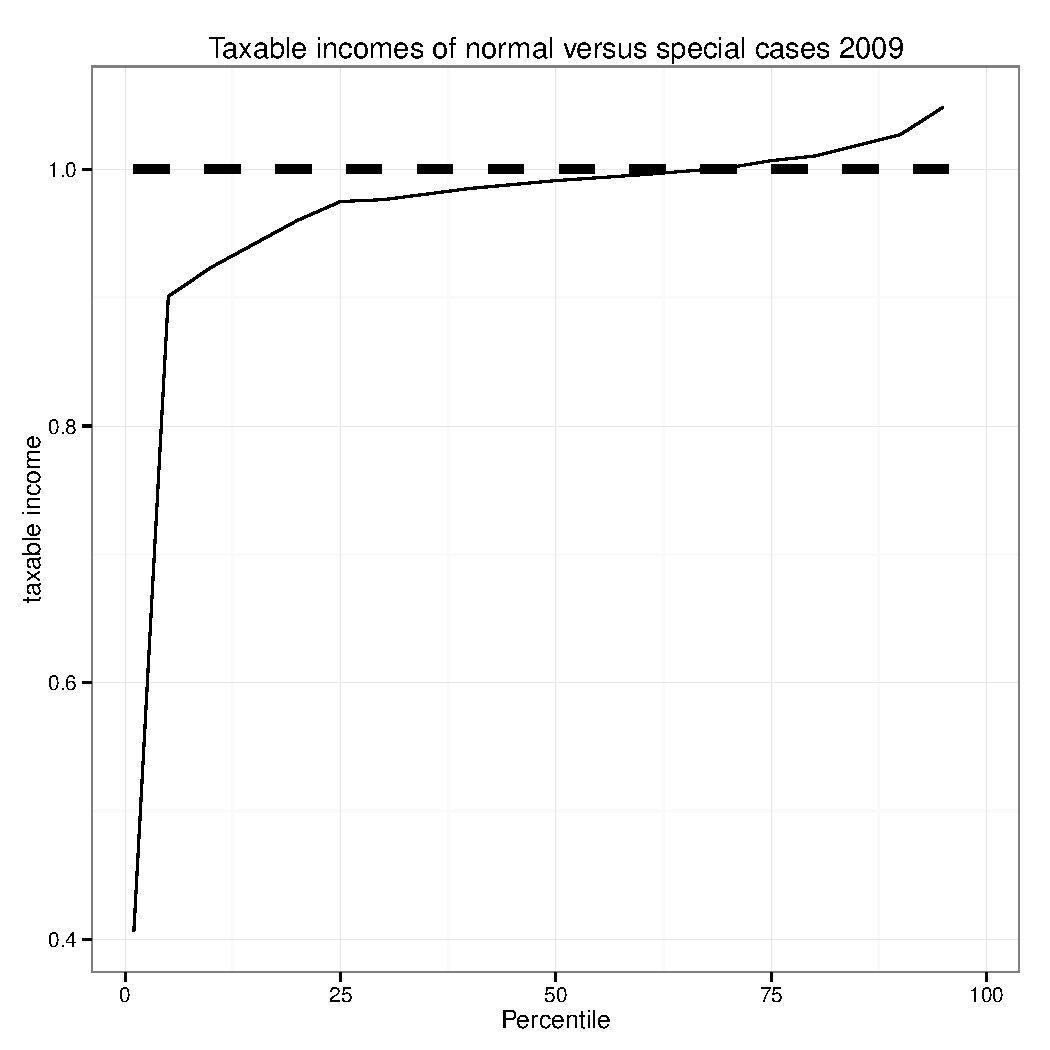
\includegraphics[width=\maxwidth]{figure/specialcases092} 

\end{knitrout}



As we can see from figure~\ref{fig:specialcases93942} and \ref{fig:specialcases092}, special cases differ strongly 
from normal cases within the low and top percentiles. Within the tax period 1993/94 the fifth percentile of 
normal cases is 15.8\% higher than the fifth percentile of the combines data while the 95\% percentile of 
normal cases is even 0.7\% lower if one leaves out special cases. This indicates special cases are very 
different from normal cases as the share of special cases is only 15.5\%.\footnote{1993/94 there were 2.76 
million tax units defined as being normal cases compared to 0.51 million special cases.}
In 2009 the situation has the same pattern. The fifth percentile of normal cases has 11\% higher taxable 
income compared to data where special cases are included. The five percent top incomes are 4.9\% higher 
within all cases compared to normal cases only. The share of special cases however decreased 
to 7.2\%.\footnote{2009: 3.42 million normal cases, 0.27 million special cases}



\emph{Income measures with and without zeros}

taxable income with and without zeros

\begin{knitrout}
\definecolor{shadecolor}{rgb}{0.969, 0.969, 0.969}\color{fgcolor}
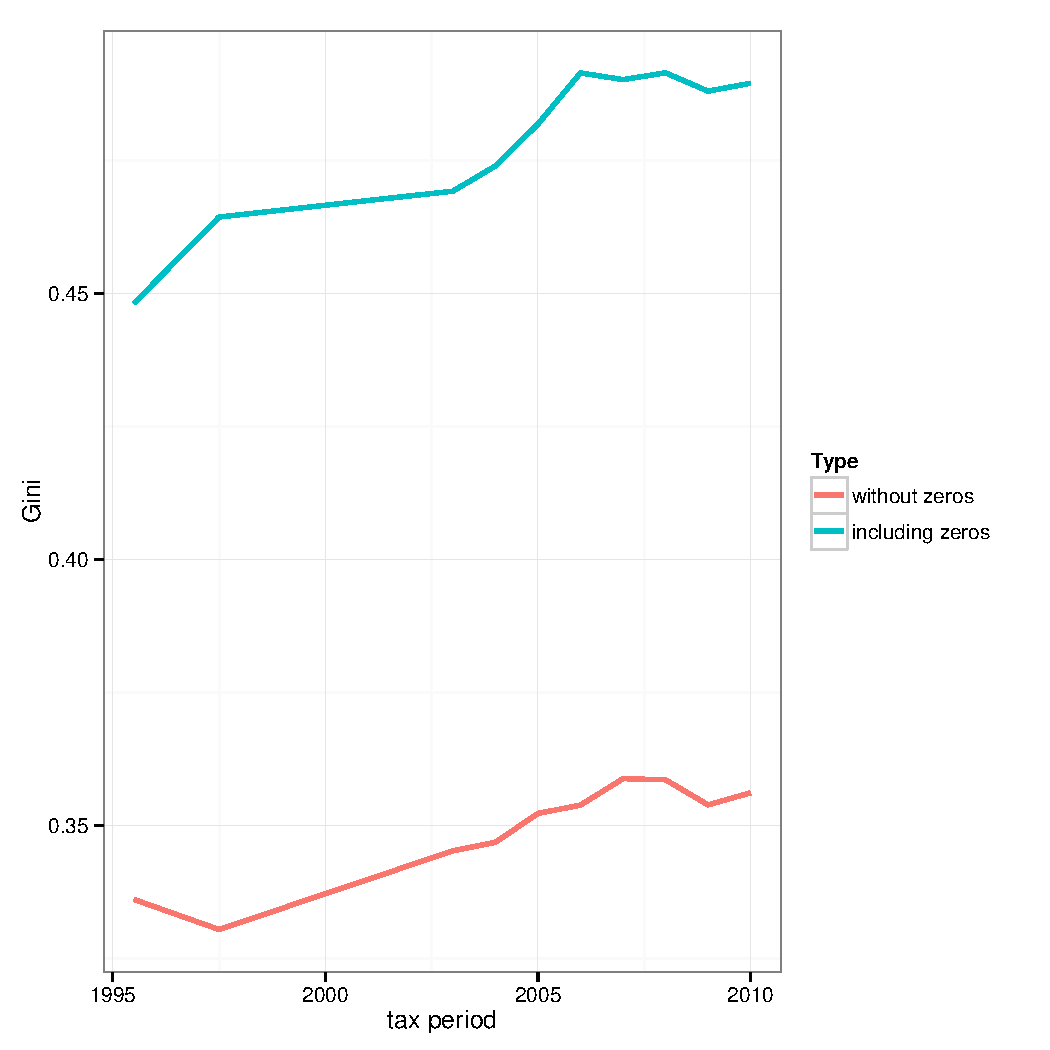
\includegraphics[width=\maxwidth]{figure/with_without_zeros1} 

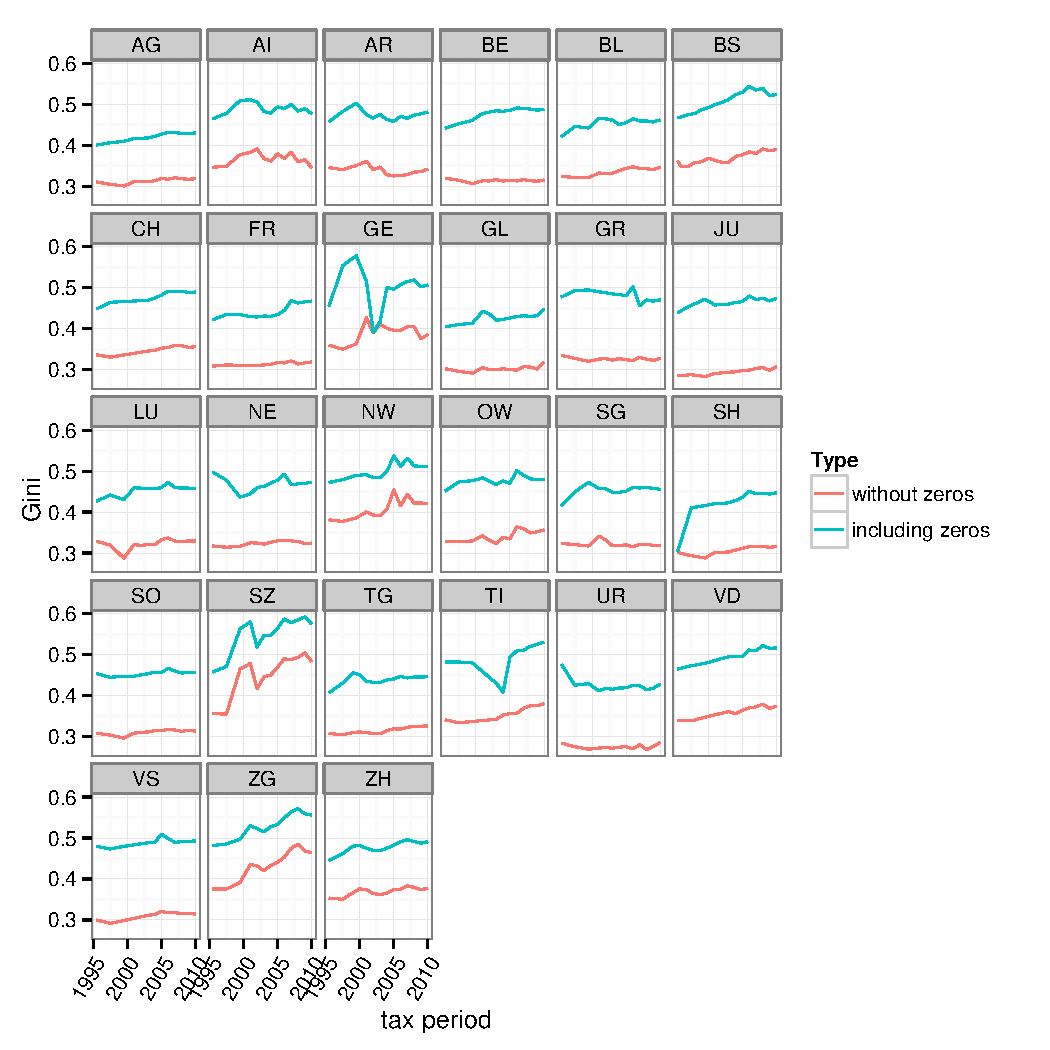
\includegraphics[width=\maxwidth]{figure/with_without_zeros2} 

\end{knitrout}


Including zeros leads to significantly higher gini coefficients. However we must keep in mind, that these might be artificially high values as we assume zero income for everyone in the zero group. We can conclude more from the graphic: the ratio between both measures seems to be quite constant although for aggregate Switzerland but there are minor deviations for multiple cantons as well as strong deviations for the cantons Geneva and Ticino. However the problems seem not to result from a shift in the zero-share over time but they are specific for the time-period when the tax system changed. 

\emph{normal and special cases}

\emph{comparison of tax-data and survey data distribution}


\subsection{Intertemporal comparison}





%%%-------------------------------------------------%%%
%%% Include discussion %%%
%%%-------------------------------------------------%%%


%%%-------------------------------------------------%%%
%%% Sub document for discussion %%%
%%%-------------------------------------------------%%%

\section{Discussion}

% Hier könnte allenfalls der Bogen zur Theorie gespannt werden 

%Methodological Main findings 
%(1) Tax data is useful because it’s possible to construct consistent measures over time for income and wealth, which is useful to asses changes over time and conducted studies about impact of structural changes.(2) Concerning accuracy of inequality tax data has advantages and shortcomings. It’s superior to survey data, because the latter is affected by non-responded bias. Tax data includes data about the whole population … [was finden wir wegen den Nullern raus] . or at least it should (tax evasion).(3) The FTA-Tax data has different shortcomings, which cannot be handled like a measure of income and wealth which (a) cannot be corrected for household size and (b) is neither a pre-transfer nor a post-transfer income measure. Therefor it’s comparability with other surveys is harsh as long as the main sources of data on inequality are based on measures, which cannot be replicated with taxable income. This FTA-Tax data problem can be handled with non-aggregated tax-data .


%Main findings for Switzerland (1) Our data suggests that income inequality overall slightly increased in Switzerland and we might distinguish three episodes: 1. Substantial increase in times of economic growth 1950 to 1974 ending with the oil crisis 2. Ups and downs from 1970 to 2000 3. Relatively steep increase in inequality in the early 2000s
%(2) Despite the recent increase, overall income inequality in Switzerland is not very high in international comparison. With respect to inequality in wealth, however, Switzerland takes a leading position in the world.
%(3) While the overall Swiss inequality remained pretty stable over decades, inequality between cantons underwent a bizarre development.

% M


%%%-------------------------------------------------%%%
%%% Include acknowledgements %%%
%%%-------------------------------------------------%%%


%%%-------------------------------------------------%%%
%%% Sub document for acknowledgement %%%
%%%-------------------------------------------------%%%

\section{Acknowledgements}

We thank Ben Jann, Robert Fluder and Tobias Fritschi for helpful comments on the article. We also like to thank Stefan Ilic for the prepartion of the data set.


%%%-------------------------------------------------%%%
%%% Include the bibliography %%%
%%%-------------------------------------------------%%%


\end{multicols}

\bibliography{bibliography/bib} 

%%%-------------------------------------------------%%%
%%% Include the appendix %%%
%%%-------------------------------------------------%%%


%%%-------------------------------------------------%%%
%%% Sub document for appendix %%%
%%%-------------------------------------------------%%%

\section{Appendix}




\end{document}
